\chapter{Konzeption und theoretische Grundlagen}
\label{cha:theoGrundlagen}

\section{Android App-Entwicklung}
Android ist ein auf dem Linux Kernel basierendes mobiles Betriebssystem. Zur
Zeit wird Android von Google entwickelt und zielt auf Geräte ab, die über einen
Touchscreen bedient werden. Dazu zählen Smartphones, Tablets und neuerdings auch
Smartwatches. Wie üblich bei auf Linux basierenden Betriebssystemen, ist auch
der Android Quellcode unter der \Fachbegriff{open source} Lizenz frei verfügbar.
Der Funktionsumfang des Betriebssystems lässt sich durch Apps beliebig
erweitern. Diese Apps können vom Benutzer aus dem \Fachbegriff{Google Play
Store} bezogen werden. Der \Fachbegriff{Play Store} stellt die zentrale App
dar, in der alle Apps katalogisiert sind die mithilfe des \Fachbegriff{Android
SDK} entwickelt wurden. \\
Das \Fachbegriff{Android Software Development Kit} bietet neben verschiedenen
Entwicklungswerkzeugen auch eine eigene Entwicklungsumgebung an. Zu den
verschiedenen Entwicklungswerkzeugen zählen unter anderem ein Debugger, die
Android Bibliotheken und ein Emulator der verschiedene mobile Endgeräte zu
Testzwecken emulieren kann. Dieser Emulator ermöglicht das Testen von Android
Applikationen falls kein physisches Gerät zur Verfügung steht. Die Kommunikation
mit physischen Geräten, beispielsweise um das Debugging von Apps auf dem Gerät
zu ermöglichen, findet über die Android Debug Bridge (ADB) statt. \\
Android Applikationen werden in \Fachbegriff{Java} entwickelt. Java ist eine 
objektorientierte Programmiersprache.
Java Quellcode wird vom Java Compiler in Bytecode umgewandelt, welcher
nicht wie bei anderen Programmiersprachen üblich direkt durch Hardware ausgeführt
wird, sondern auf einer virtuellen Maschine (der Java Virtual Machine) läuft.
Dies sorgt für die oft beworbene Plattformunabhängigkeit von Java. Ob Windows,
Mac, Linux oder mobile Betriebssysteme wie z.B Android, das Java Prinzip „Write
once run anywhere“ bringt Java auf mehr als 50 Mio. PCs und Milliarden von verschiedensten
Geräten weltweit.\footcite{sierra2006} \\
Die Entwicklung mit dem Android SDK unterscheidet sich nur an manchen Stellen
von klassischer Java Entwicklung. Viele native Java Bibliotheken können auch in
der Android Entwicklung eingesetzt werden. Die Entwicklung von Oberflächen
unterschiedet sich jedoch etwas von der klassischen Oberflächenentwicklung mit
\Fachbegriff{Java Swing}. Android Oberflächen werden in sogenannte
\Fachbegriff{Activities} unterteilt. Üblicherweise ist jeder
\Fachbegriff{Activity} eine bestimmte Oberfläche zugeordnet. Mithilfe der
verschiedenen \Fachbegriff{Activities} wird in erster Linie die Navigation
innerhalb der App gesteuert. Die \Fachbegriff{Activities} reagieren auf Gesten
und Tastendrücke des Benutzers. Sollte also ein Benutzer beispielsweise den
\Fachbegriff{Zurück} Button auf seinem Gerät drücken, so wechselt die App auf
die zuvor angezeigte \Fachbegriff{Activity}. \Fachbegriff{Activities} können
sich auch gegenseitig aufrufen und stellen somit
den Navigationsfluss innerhalb der App sicher.\footcite{künneth2012android}

\section{Eingesetzte Technologien}
\subsection{Jsoup}
Um die Informationen im readmore.de Forum, also verschiedene Foren und Beiträge,
auszulesen, wird die Java Bibliothek \Fachbegriff{jsoup} auf der
Serverseite eingesetzt.
\Fachbegriff{jsoup} ist eine Bibliothek mit der es möglich ist, HTML Dateien zu
parsen und die enthaltenen Informationen zu extrahieren. \Fachbegriff{jsoup}
bietet hierzu die Möglichkeit die Baumstruktur des eingelesenen HTML Dokuments
zu durchlaufen und beispielsweise nach bestimmten Attributen zu filtern. Dazu
bietet die Bibliothek mit der sogenannten \Fachbegriff{Selektor Syntax} eine
Manipulationssprache um bestimmte Elemente im \Fachbegriff{DOM} des HTML
Dokument zu selektieren. Ein \Fachbegriff{DOM} ist in diesem Kontext die 
Baumstruktur in der das HTML Dokument strukturiert ist. \\
\subsection{Restlet}
Damit der Server auch von außen über HTTP Requests erreichbar ist, wurde das
Framework \Fachbegriff{Restlet} eingesetzt um eine \Fachbegriff{RESTful}
Serverkomponente bereit zu stellen. Das Programmierparadigma Representational
State Transfer (kurz: REST) beschreibt eine Serverkomponente die lediglich
unveränderte Seiteninhalte zum Abruf bereitstellt. Die Kommunikation mit dieser
Serverkomponente erfolgt über verschiedene HTTP-Methoden. Um beispielsweise
Daten vom Server abzurufen wird die Methode \Fachbegriff{GET} verwendet. Der Zustand am Server
wird dadurch nicht verändert. Restlet bringt eine fertige Serverkomponente mit
die nur noch an einem Port registriert werden muss. Über einen
\Fachbegriff{Router} werden dann Adressen verteilt die auf einzelne
\Fachbegriff{Restlets} verweisen. Wird also die URL eines \Fachbegriff{Restlets}
aufgerufen, reagiert das \Fachbegriff{Restlet} mit seiner Methode
\Code{handle()} auf die Anfrage. Dort werden dann die eventuellen Parameter des
GET-Requests ausgelesen, die Anfrage wird verarbeitet und anschließend wird die
angeforderte Ressource zurückgegeben. Nachfolgend ein Beispiel einer einfachen
\Fachbegriff{Restlet}-Serverkomponente mit einem Restlet.
\begin{lstlisting}[caption=Die Serverkomponente, label=komponente]
public class ReadmoreServer extends Application {
	private static ThreadsRestlet threadsRestlet;
	private static ForumRestlet forumRestlet;
	private static BeitragRestlet beitragRestlet;
	static {
		threadsRestlet = new ThreadsRestlet();
		forumRestlet = new ForumRestlet();
		beitragRestlet = new BeitragRestlet();
	}
	public static void main(String[] args) throws Exception {
		Component component = new Component();
		component.getServers().add(Protocol.HTTP, 8182);
		ReadmoreServer server = new ReadmoreServer();
		component.getDefaultHost().attach("", server);
		component.start();
	}
	public Restlet createInboundRoot() {
	    Router router = new Router(getContext());
	    router.attach("/threads", threadsRestlet);
	    router.attach("/forum", forumRestlet);
	    router.attach("/beitrag", beitragRestlet);
	    return router;
	  }
}
\end{lstlisting}
Wie in \ref{komponente} zu sehen, hört die Serverkomponente auf einen bestimmten
Port. In der Methode \Code{createInboundRoot()} wird mithilfe des \Code{Router}
die Adressen auf die die einzelnen Restlets reagieren festgelegt. Nachfolgend
ein einfaches \Fachbegriff{Restlet}
\begin{lstlisting}[caption=Ein einfaches Restlet, label=restlet]
public class ForumRestlet extends Restlet {
	@Override
    public void handle(Request request, Response response) {
		List<Forum> forum = getForum();
        String message = null;
        Gson gson = new Gson();
        message = gson.toJson(forum);
        response.setEntity(message, MediaType.TEXT_PLAIN);
    }
	private List<Forum> getForum() {
		ForenParser tp = new ForenParser();
		return tp.getForen();
	}
}
\end{lstlisting}
Die Methode \Code{handle(Request request, Response response)} legt beim Aufruf
des Restlets die \Fachbegriff{Response}, also die Antwort des Servers fest die
beim Aufruf zurückgegeben wird.
\subsection{Gson}
Das von Google entwickelte Framework \Fachbegriff{Gson} bietet die Möglichkeit
Java-Objekte vollautomatisch in das \Fachbegriff{JSON}-Format zu übertragen und
umgekeht \Fachbegriff{JSON}-Objekte in existierende Java-Objekte zu
transferieren.\footnote{https://sites.google.com/site/gson/gson-user-guide} 
\Fachbegriff{Gson} wird auf der Serverkomponente zur Erstellung der Antwort auf
GET Anfragen verwendet. 
\section{Konzeption des Servers}
Die Serverkomponente der Readmore App dient in erster Linie dem Auslesen der
sichtbaren Informationen im Forum von readmore. Dazu gehören die verschiedenen
Foren die in verschiedene Kategorien unterteilt sind, die Threads, also die
Einträge in jedem gewählten Forum und die einzelnen Beiträge auf jeder Seite
eines gewünschten Threads. 
\begin{figure*}[!htbp]
\centering
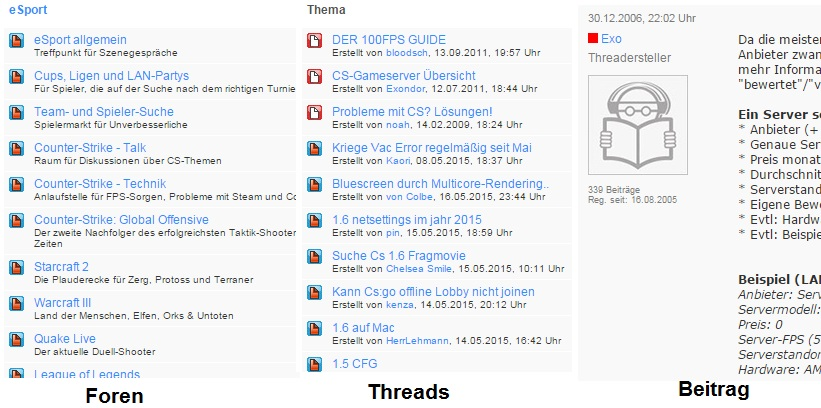
\includegraphics[width=\textwidth]{Bilder/ftb.jpg}
\caption[Foren, Threads und Beiträge auf Readmore]{Foren, Threads und Beiträge auf Readmore\protect\footnote{eigene Darstellung.} }
\label{dminfo}
\end{figure*}
Die App soll also nicht direkt mit readmore.de kommunizieren sondern bekommt
alle zur Anzeige des Forums relevanten Informationen in einem schnell zu
verarbeitenden Format. Dieses Vorgehen legt das aufwendige traversieren durch
den HTML-Code von readmore.de auf den Server um, und spart somit wertvolle
Ressourcen des Mobilgeräts ein.
\section{Anforderungen an die Oberfläche}
Use Cases, Mockups der Oberfläche usw.